%%
%% This is file `sample-sigconf.tex',
%% generated with the docstrip utility.
%%
%% The original source files were:
%%
%% samples.dtx  (with options: `sigconf')
%%
%% IMPORTANT NOTICE:
%%
%% For the copyright see the source file.
%%
%% Any modified versions of this file must be renamed
%% with new filenames distinct from sample-sigconf.tex.
%%
%% For distribution of the original source see the terms
%% for copying and modification in the file samples.dtx.
%%
%% This generated file may be distributed as long as the
%% original source files, as listed above, are part of the
%% same distribution. (The sources need not necessarily be
%% in the same archive or directory.)
%%
%% The first command in your LaTeX source must be the \documentclass command.
\documentclass[sigconf]{acmart}


% Packages
\usepackage{amsfonts}
\usepackage{amsmath}
\usepackage{graphicx}
\usepackage{hyperref}
\usepackage{float}
\usepackage{pgfplots}
\usepgfplotslibrary{fillbetween}
\usepackage[pdf]{graphviz}
\usepackage{tikz}
\usepackage{natbib}

\usepackage{booktabs}
\usepackage{pifont}
\usepackage{fontawesome}

\newcommand{\wmark}{\textcolor{orange}{\ding{45}}}
\newcommand{\cmark}{\textcolor{green!80!black}{\ding{51}}}
\newcommand{\xmark}{\textcolor{red}{\ding{55}}}

\usepackage{multicol}

%% NOTE that a single column version may be required for
%% submission and peer review. This can be done by changing
%% the \doucmentclass[...]{acmart} in this template to
%% \documentclass[manuscript,screen]{acmart}
%%
%% To ensure 100% compatibility, please check the white list of
%% approved LaTeX packages to be used with the Master Article Template at
%% https://www.acm.org/publications/taps/whitelist-of-latex-packages
%% before creating your document. The white list page provides
%% information on how to submit additional LaTeX packages for
%% review and adoption.
%% Fonts used in the template cannot be substituted; margin
%% adjustments are not allowed.
%%
%%
%% \BibTeX command to typeset BibTeX logo in the docs
\AtBeginDocument{%
  \providecommand\BibTeX{{%
    \normalfont B\kern-0.5em{\scshape i\kern-0.25em b}\kern-0.8em\TeX}}}

%% Rights management information.  This information is sent to you
%% when you complete the rights form.  These commands have SAMPLE
%% values in them; it is your responsibility as an author to replace
%% the commands and values with those provided to you when you
%% complete the rights form.
\setcopyright{acmcopyright}
\copyrightyear{2018}
\acmYear{2018}
\acmDOI{10.1145/1122445.1122456}

%% These commands are for a PROCEEDINGS abstract or paper.
\acmConference[Woodstock '18]{Woodstock '18: ACM Symposium on Neural
Gaze Detection}{June 03--05, 2018}{Woodstock, NY}
\acmBooktitle{Woodstock '18: ACM Symposium on Neural Gaze Detection,
  June 03--05, 2018, Woodstock, NY}
\acmPrice{15.00}
\acmISBN{978-1-4503-XXXX-X/18/06}


\newcommand{\seqWord}{Seq \langle Word \rangle}
\newcommand{\distSeqWord}{Dist\langle \seqWord  \rangle}

%%
%% Submission ID.
%% Use this when submitting an article to a sponsored event. You'll
%% receive a unique submission ID from the organizers
%% of the event, and this ID should be used as the parameter to this command.
%%\acmSubmissionID{123-A56-BU3}

%%
%% The majority of ACM publications use numbered citations and
%% references.  The command \citestyle{authoryear} switches to the
%% "author year" style.
%%
%% If you are preparing content for an event
%% sponsored by ACM SIGGRAPH, you must use the "author year" style of
%% citations and references.
%% Uncommenting
%% the next command will enable that style.
%%\citestyle{acmauthoryear}

%%
%% end of the preamble, start of the body of the document source.
\begin{document}

%%
%% The "title" command has an optional parameter,
%% allowing the author to define a "short title" to be used in page headers.
  \title{Symbolic Automata for Code Search}

%%
%% The "author" command and its associated commands are used to define
%% the authors and their affiliations.
%% Of note is the shared affiliation of the first two authors, and the
%% "authornote" and "authornotemark" commands
%% used to denote shared contribution to the research.
  \author{Breandan Considine, Xujie Si, Jin Guo}
  \email{{breandan.considine, xujie.si, jguo}@mail.mcgill.ca}
  \affiliation{%
    \institution{McGill University}
  }

%%
%% By default, the full list of authors will be used in the page
%% headers. Often, this list is too long, and will overlap
%% other information printed in the page headers. This command allows
%% the author to define a more concise list
%% of authors' names for this purpose.
% \renewcommand{\shortauthors}{Trovato and Tobin, et al.}

%%
%% The abstract is a short summary of the work to be presented in the
%% article.
  \begin{abstract}
    Neural networks are increasingly capable of performing end-to-end document comprehension and retrieval. Training these models, however, is equivalent to reading every document in the dataset and tends to produce models which are (1) uninterpretable, (2) disregards user intent and (3) modification is expensive and requires retraining. We would like to produce a model which can retrieve contextually relevant search results based on user intent, available at inference time, and whose query model can be interpreted and modified by the user. The model used to express intent is a symbolic automaton: the model reads the user's context and produces a default query, which the user can modify to filter various types of results.
  \end{abstract}

%% A "teaser" image appears between the author and affiliation
%% information and the body of the document, and typically spans the
%% page.
% \begin{teaserfigure}
%   \includegraphics[width=\textwidth]{sampleteaser}
%   \caption{Seattle Mariners at Spring Training, 2010.}
%   \Description{Enjoying the baseball game from the third-base
%   seats. Ichiro Suzuki preparing to bat.}
%   \label{fig:teaser}
% \end{teaserfigure}

%%
%% This command processes the author and affiliation and title
%% information and builds the first part of the formatted document.
  \maketitle

  \section{Introduction}\label{sec:introduction}

  Humans are adept information foraging agents. We can quickly find relevant information in a large corpus by recognizing and following textual landmarks. Software projects are composed of a variety of semi-structured documents containing many clues where relevant information may be found. In this work, we learn a grammar from a model trained on software artifacts like source code and documentation, in order to facilitate common programming tasks such as code search, completion, or knowledge discovery.

%Our work broadly falls under the umbrella of text-based reinforcement learning. Prior literature falls under two categories: natural or formal language. Reinforcement learning (RL) in the natural domain typically focuses on question answering~\citep{buck2017ask, chen2019reinforcement}, or interactive text games~\citep{he2015deep,ammanabrolu2018playing,narasimhan2015language,guo2020interactive,ammanabrolu2020graph}. RL techniques have begun to show promising results for program synthesis~\citep{ellis2019write, johnson2020learning, chen2020program}. Our work falls at the intersection of these two domains.

  Early work in program learning realized the importance of graph-based representations~\citep{allamanis2017learning}, however explicit graph construction requires extensive feature-engineering. More recent work in program synthesis has explored incorporating a terminal~\citep{ellis2019write}, graphical~\citep{walke2020learning} or other user interface to explore the space of valid programs, however do not consider the scope or variety of artifacts in a software project. Others have shown the feasibility of learning a local graph~\citep{johnson2020learning} from source code, but still require an explicit parser to form the initial graph and adaption to settings where style, terminology and document structure vary remains a challenge.


  Imagine a newly-hired developer, who has programming experience, but no prior knowledge about a closed-source project. She receives access to the team's Git repository and is assigned her first ticket: Fix test broken by \texttt{0fb98be}. After locating the commit and becoming familiar with the code, she queries StackOverflow, discovers a relevant solution, copies the code into the project, makes a few edits, presses run, and the test passes.

  In order to accomplish a similar task, an information-seeking agent must be able to explore a local database for information, construct a query, and search a remote database. Similar to a human developer, it might traverse the project to gather information, taking note of various keywords, APIs and design patterns. While traversing the project, the model constructs a project-specific knowledge graph, which it uses to locate other relevant artifacts written by authors who solved the same problem.

%\begin{figure*}
%  \centering
%  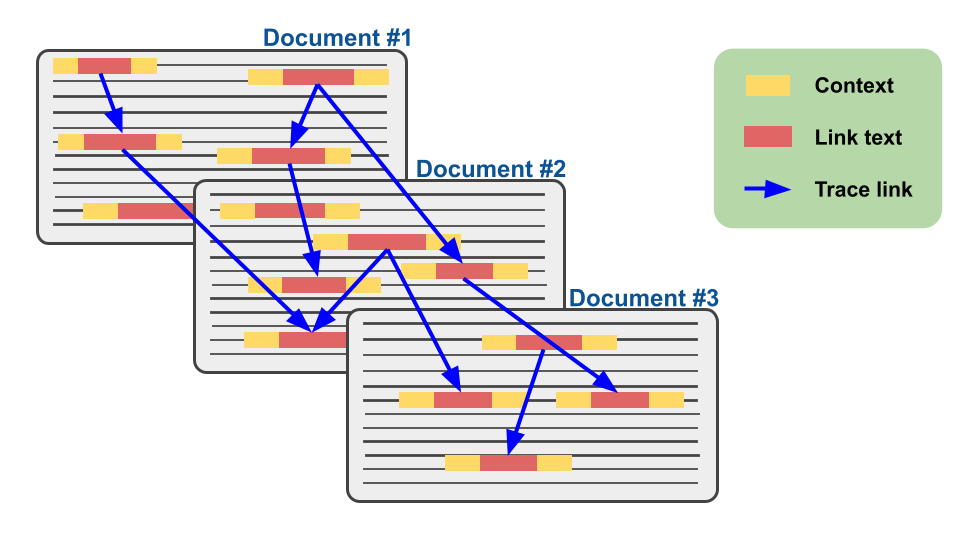
\includegraphics[width=0.8\textwidth]{use_graph}
%  \caption{Software projects consist of many documents which share common references. These references form an entity alignment graph, with vertices decorated by the surrounding context, and edges by the relation type, e.g. exact duplicate, fuzzy match or synthetic relation (learned or engineered).}
%\end{figure*}

%During evaluation, we measure task performance across search strategies. Depending on the task in question, various loss functions are possible, from a simple string distance metric over a masked code fragment, to more complex properties (e.g. the presence or absence of errors, or some internal state of the REPL) that must be satisfied by interacting with the runtime environment. Many program analysis and repair tasks are also possible, such as defect, duplicate or vulnerability detection and correction.


  \section{Prior literature}\label{sec:prior-literature}

  Prior work in the code search literature explores the text-to-code~\citep{husain2019codesearchnet} setting, where queries are typically considered to be a short sequence composed by the user, or code-to-code~\citep{kim2018facoy} setting where the query takes the form of a code snippet. Model performance typically evaluated using mean reciprocal rank (MRR), mean average precision (MAP), normalized discounted cumulative gain (NDCG), precision and recall at top N-results (P/R@N), or similar metrics. Although some~\citep{asyrofi2020ausearch} do incorporate other features from the local document, none however, consider the query in the context of a broader project. The ability to align contextual features from the surrounding project, we argue, is essential to delivering semantically relevant search results.

% {
% \renewcommand{\arraystretch}{1.5}
% \begin{table}[H]
%   \small
%   \begin{tabular}{lllc}
%     Name & Type & Key contribution & Evaluation method \\
%     \hline
%     \href{https://github.com/breandan/gym-fs}{\textsc{Our Work}} & Either-to-Either & Learning to search & Prediction accuracy \\
%     \href{https://core.ac.uk/download/pdf/162022846.pdf#page=7}{\textsc{FaCoY}}~\citep{kim2018facoy} & Code-to-code & Similarity search & MRR \\
%     \href{https://www.jameskoppel.com/files/papers/yogo-preprint.pdf#page=11}{\textsc{Yogo}}~\cite{premtoon2020semantic}     & Code-to-code & Equational reasoning & Case study \\
%     \href{https://arxiv.org/pdf/1909.09436.pdf#page=5}{\textsc{CSNet}}~\citep{husain2019codesearchnet}     & Text-to-code & Big code benchmark & MRR \\
%     \href{https://arxiv.org/pdf/1812.01158.pdf#section.5}{\textsc{Aroma}}~\citep{luan2019aroma}     & Code-to-code & Structural Search& Recall@N \\
%     \href{https://raw.githubusercontent.com/mhilmiasyrofi/AUSearch/master/SANER_2020_AUSearch.pdf}{\textsc{AUSearch}}~\citep{asyrofi2020ausearch}     & Code-to-code & Type resolver & Highlight accuracy \\

%     \href{https://arxiv.org/pdf/1905.03813.pdf#section.4}{\textsc{Cambronero}}~\citep{cambronero2019deep}     & Text-to-code & Semantics & Answered@N \\
%     \href{https://guxd.github.io/papers/deepcs.pdf#section.5}{\textsc{DeepCS}}~\citep{gu2018deep}     & Text-to-code & Deep learning & FRank, *@N, MRR \\
%     \href{https://www.cs.sjtu.edu.cn/~zhonghao/paper/Lancer.pdf}{\textsc{Lancer}}~\citep{zhou2019lancer}     & Code-to-code & BERT embedding & HitRate@k, MRR \\
%   \end{tabular}
%   \caption{\label{tab:ad_comparison} Comparison of existing code search tools.}
% \end{table}
% }

  Although we draw some inspiration from the duplicate detection literature, their work presumes the code was intentionally duplicated or modified but is essentially identical in form or function. In contrast, our work seeks to help users discover artifacts which predictive of as-yet-incomplete code. By aligning salient features from the surrounding document and project graph, we approximate the notion of semantic similarity, without requring a language-specific parser like some methods~\citep{cambronero2019deep} do, and can more easily adapt to settings where the language and project structure varies.

  Furthermore, unlike prior work, our work considers the surrounding project and related artifacts. Instead of parsing their contents explicitly, which may be computationally intractable, we allow the agent to construct the graph organically by exploring the filesystem, then extract a query.

  \section{Method}\label{sec:method}

  Do language models learn to recognize patterns in source code? If so, what kinds? A longstanding research area in software engineering tries to extract idioms from large software repositories. Likewise, a longstanding goal of neural program synthesis is compositional generalization. Both currently require designing a feature representation that “selects” for a specific kind of invariance — for example, structural similarity measures naming-invariance, and program understanding requires an intermediate representation.

% For example, suppose we are given a string of text in a foreign language:

% Ribbit bleep bloop ribbet

% Perhaps the “bleep bloop” is a proper name, which could be replaced with any other without changing the meaning:

% Ribbit flip flop ribbet

% Or perhaps flip/flop changes the meaning drastically. How do we know from examples alone?

  Imagine that we have a stochastic language model that takes a sequence and emits a distribution over sequences:

  $LM: \seqWord  \rightarrow \distSeqWord $

  But how do we obtain LM in the first place? A good language metamodel then, would produce language models that tend to generalize, or align with user preferences:

  $LMM: \distSeqWord \rightarrow \texttt{LM}$

  For many computational languages, the number of models that explain our data far outnumber the size of the dataset, e.g. depending on the language complexity, there can be an exponential, or super-exponential number of models that exactly describe the data. If we wish to consider models that approximate the data, the number of models is effectively infinite. How do we form a distribution over models we cannot even enumerate? For small trees, it may be possible to perform beam-search, but for any reasonably sized query, we simply cannot enumerate all possibilities.

  Furthermore, models typically average across all authors, needs, intents and situations. Language model designers are forced to compress human needs into the model training algorithm, which does not work very well. Effectively, we select a higher-order model which produces models that tend to align with human-selected priors. Since these priors are often hard to translate, there must be more human input during the design process. Most of these preferences are incorporated implicitly during the meta model design phase in the dataset selection and feature design.

  $LMM: (Intent) \times (Training Data) \rightarrow LM$

  Rather than push all the needs and intent into the model training, we argue that these needs should be incorporated into the model at inference time. This is essentially the goal of meta learning, to factorize these probabilities into separate inputs.

  $LM: \seqWord \times (Intent) \rightarrow \distSeqWord$

  If we want to be able to make better code assistants, we need to incorporate the preferences of the human at runtime. To develop more reusable and human adaptive models, we need a way to train a model that can incorporate the user’s preferences at runtime. Instead of trying to anticipate the users needs a priori, we need to be able to produce a model that can take some input from the user (say a query) and emit an answer:

  $LM: ( \seqWord ) \times (Query) \rightarrow \distSeqWord $

% So the user can feed a query and depending on the query, the model will adjust the output distribution depending on its contents.


  In our work, we explore the extent to which recent language models trained on source code learn regularities they were not explicitly designed to represent. We analyze four or five different language models, and compare their zero-shot generalization on synthetically-generated patterns. We generate code snippet pairs corresponding to manually-identified idioms, and measure inter-rater agreement between language models. Each model rates the similarity between manually-designed code snippets which vary along specific dimensions. Each model represents a human rater, which compares two code snippets for similarity.

  We fetch a dataset of repositories sampled repositories on GitHub, containing a mixture of filetypes representing source code and natural language artifacts. From each repository, we index all substrings of every line in every file using a variable height radix tree producing a multimap of $\texttt{kwdIndex: String -> List<Location<F, O>>}$ of $\texttt{String}$  queries to file-offset pairs. We also encode CodeBERT~\citep{feng2020codebert} sequence embeddings to substrings $\texttt{knnIndex: Vector -> Location<F, O>}$ using a Hierarchial Navigavble Small World Graph~\citep{malkov2018efficient} (HNSWG).

  \begin{figure}[H]
    \centering
    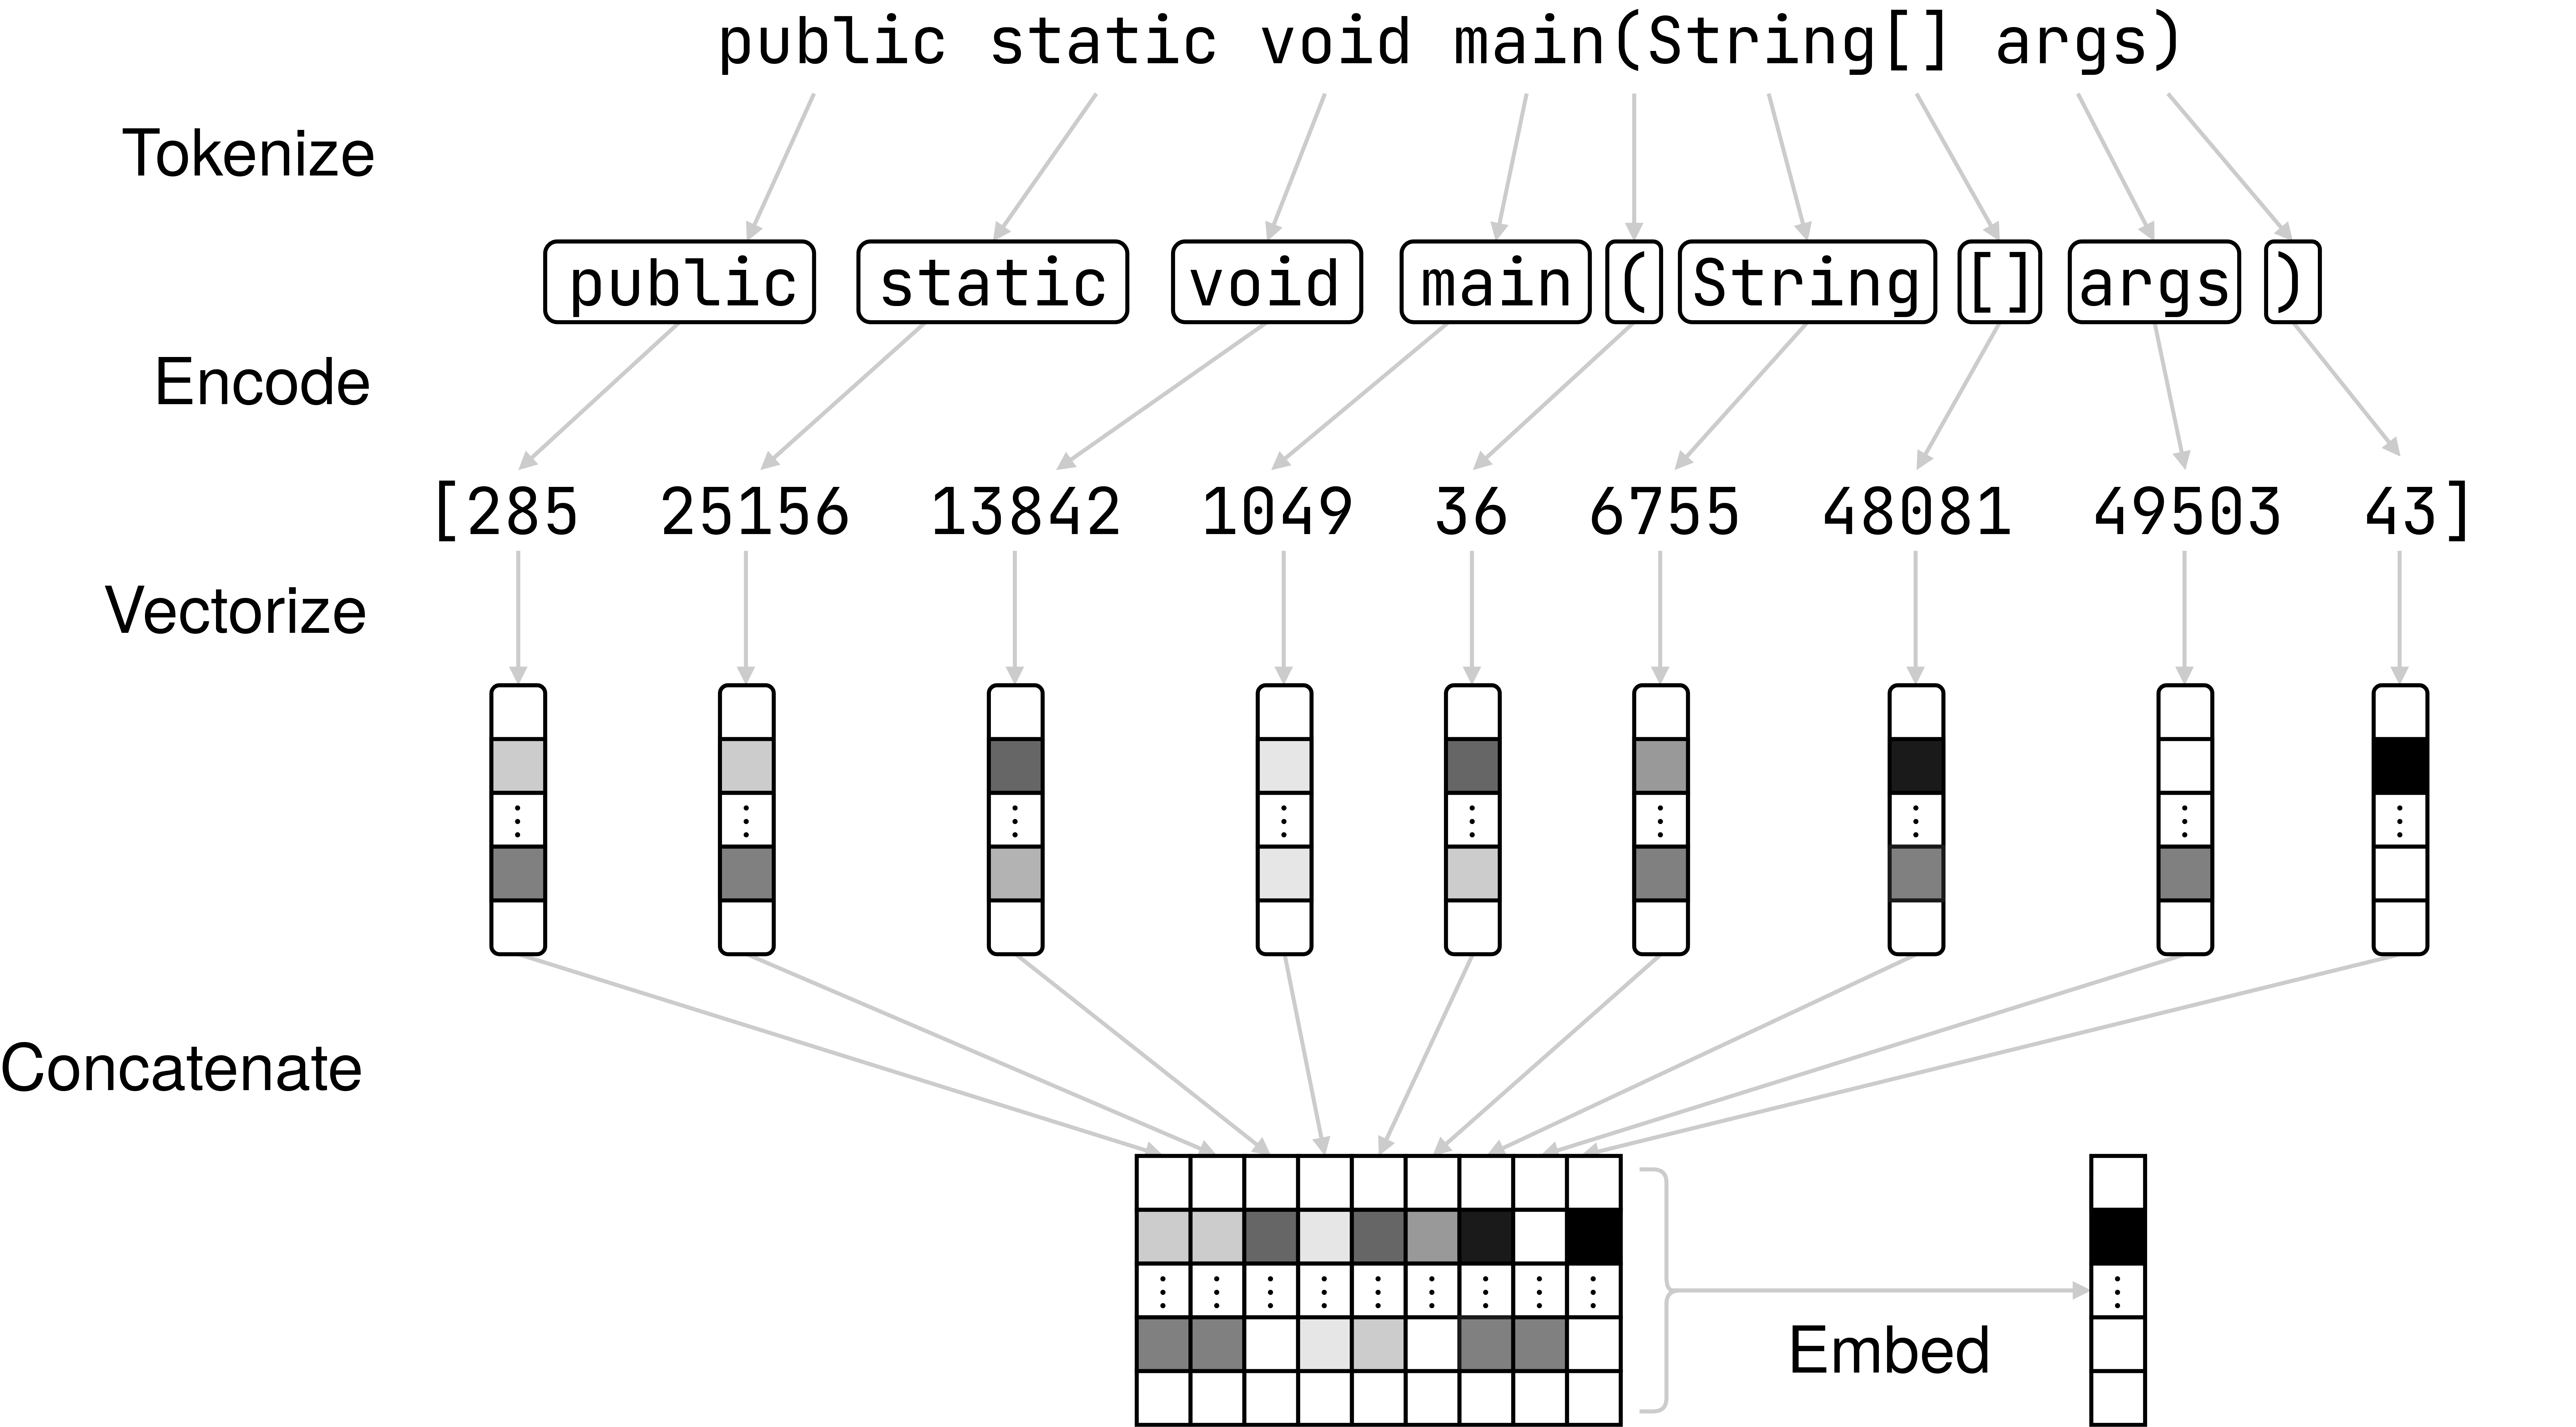
\includegraphics[width=0.40\textwidth]{figs/bert_embedding}
    \caption{CodeBERT takes a unicode sequence and emits a vector sequence, which we accumulate into a single vector.}
    \label{fig:bert}
  \end{figure}

  For each token in a string, CodeBERT emits a length-768 vector, so a line with $n$ tokens produces a matrix of shape $\mathbb R^{768 \times (n + 1)}$, the first column of which contains the final hidden layer activations. We concatenate the CodeBERT sequence `\texttt{<s>}' and using the source tokens, encode and vectorize the encoded sequence using the vocabulary, then take the first row as our sequence embedding as depicted in Fig.~\ref{fig:bert}. In \S~\ref{sec:results}, we compare various distance-metrics to fetch the nearest sequence embeddings in our database and compare precision and recall across various types of distance metrics.

  \begin{figure}[H]
    \centering
    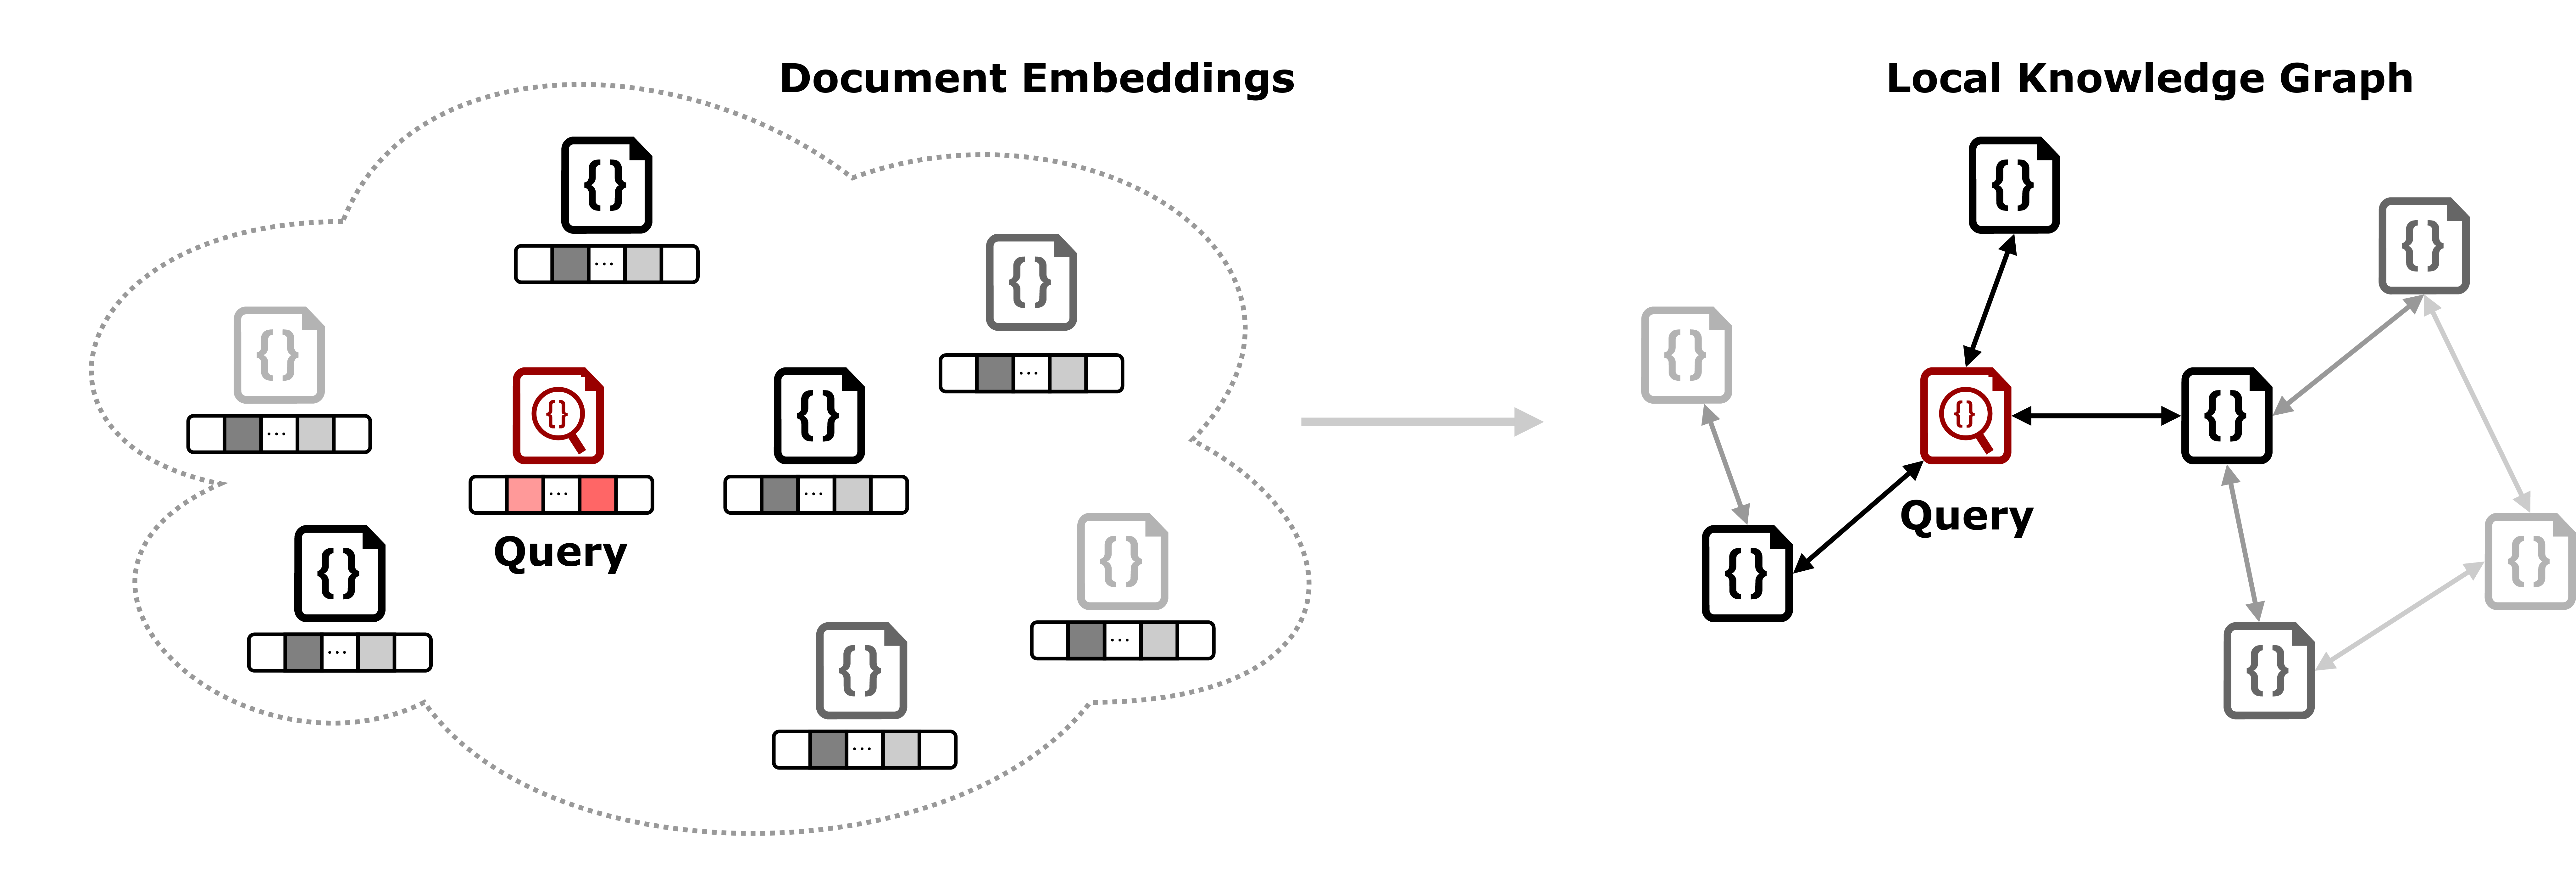
\includegraphics[width=0.4\textwidth]{figs/latent_kg}
    \caption{To compute our query neighborhood, we traverse the HNSWG up to max depth $d$, i.e. $d=1$ fetches the neighbors, $d=2$ fetches the neighbors-of-neighbors, and $d=3$ fetches the neighbors-of-neighbors-of-neighbors.}
    \label{fig:de2kg}
  \end{figure}

  For a given query and context, we first compute the context embedding and using a distance metric, fetch the k-nearest neighboring documents in latent space, forming the depth-1 nodes in our graph, then repeat this procedure recursively, pruning with a beam search heuristic based on the total path length in latent space. This procedure is depicted in Fig.~\ref{fig:de2kg}.

  \begin{figure}[H]
    \centering
    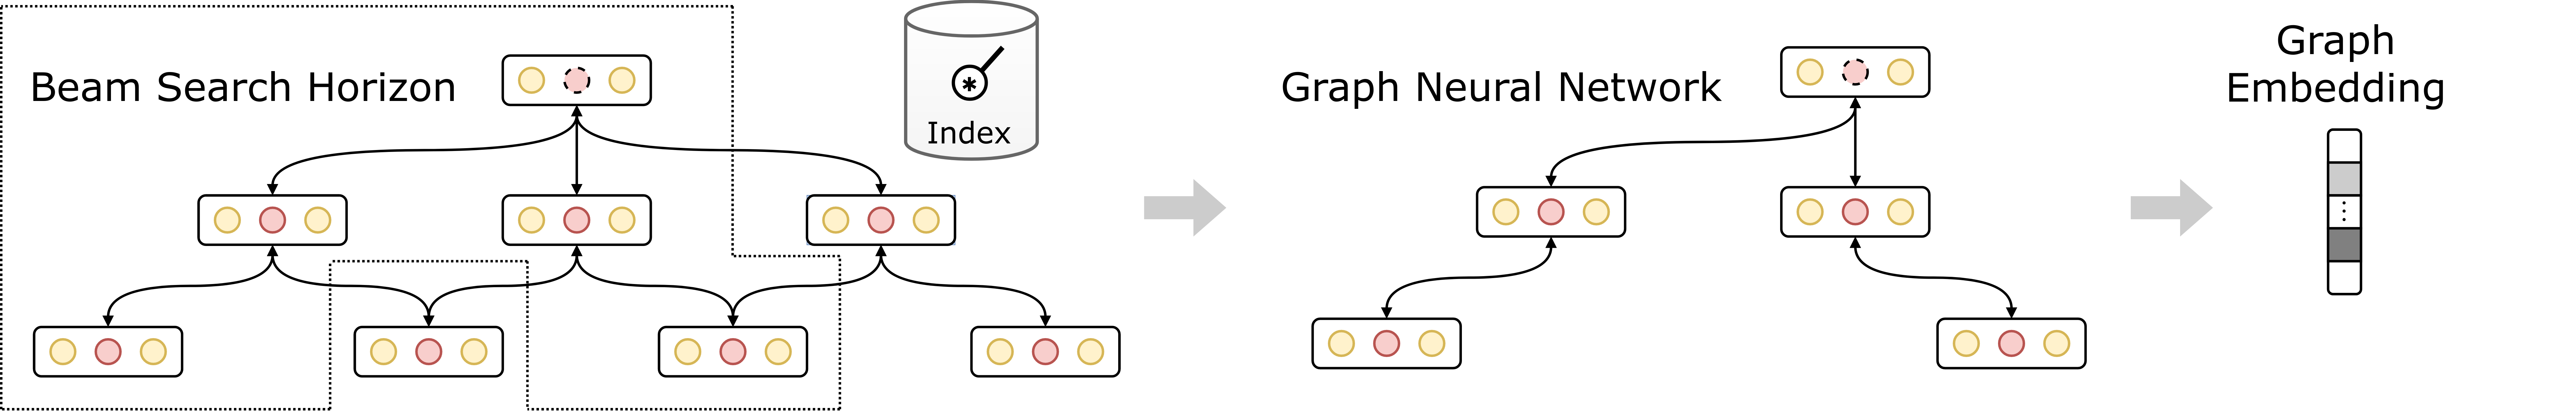
\includegraphics[width=0.4\textwidth]{figs/architecture}
    \caption{Unlike language models which directly learn the data distribution, our model is designed to query an unseen database only available at test time. The model scores and selectively expands a subset of promising results within the database using a beam search heuristic, then runs message passing over the resulting graph to obtain the final task prediction.}
    \label{fig:architecture}
  \end{figure}

  Consider the depth-1 beam search procedure (Fig. ~\ref{fig:pipeline}): We can use either vector search or keyword search to perform the context expansion, although vector search has the disadvantage of needing to rebuild the vector embedding index at each step during training. Keyword search is comparatively cheaper, as it only needs to build once for each repo on MiniGithub.

  \begin{figure}[H]
    \centering
    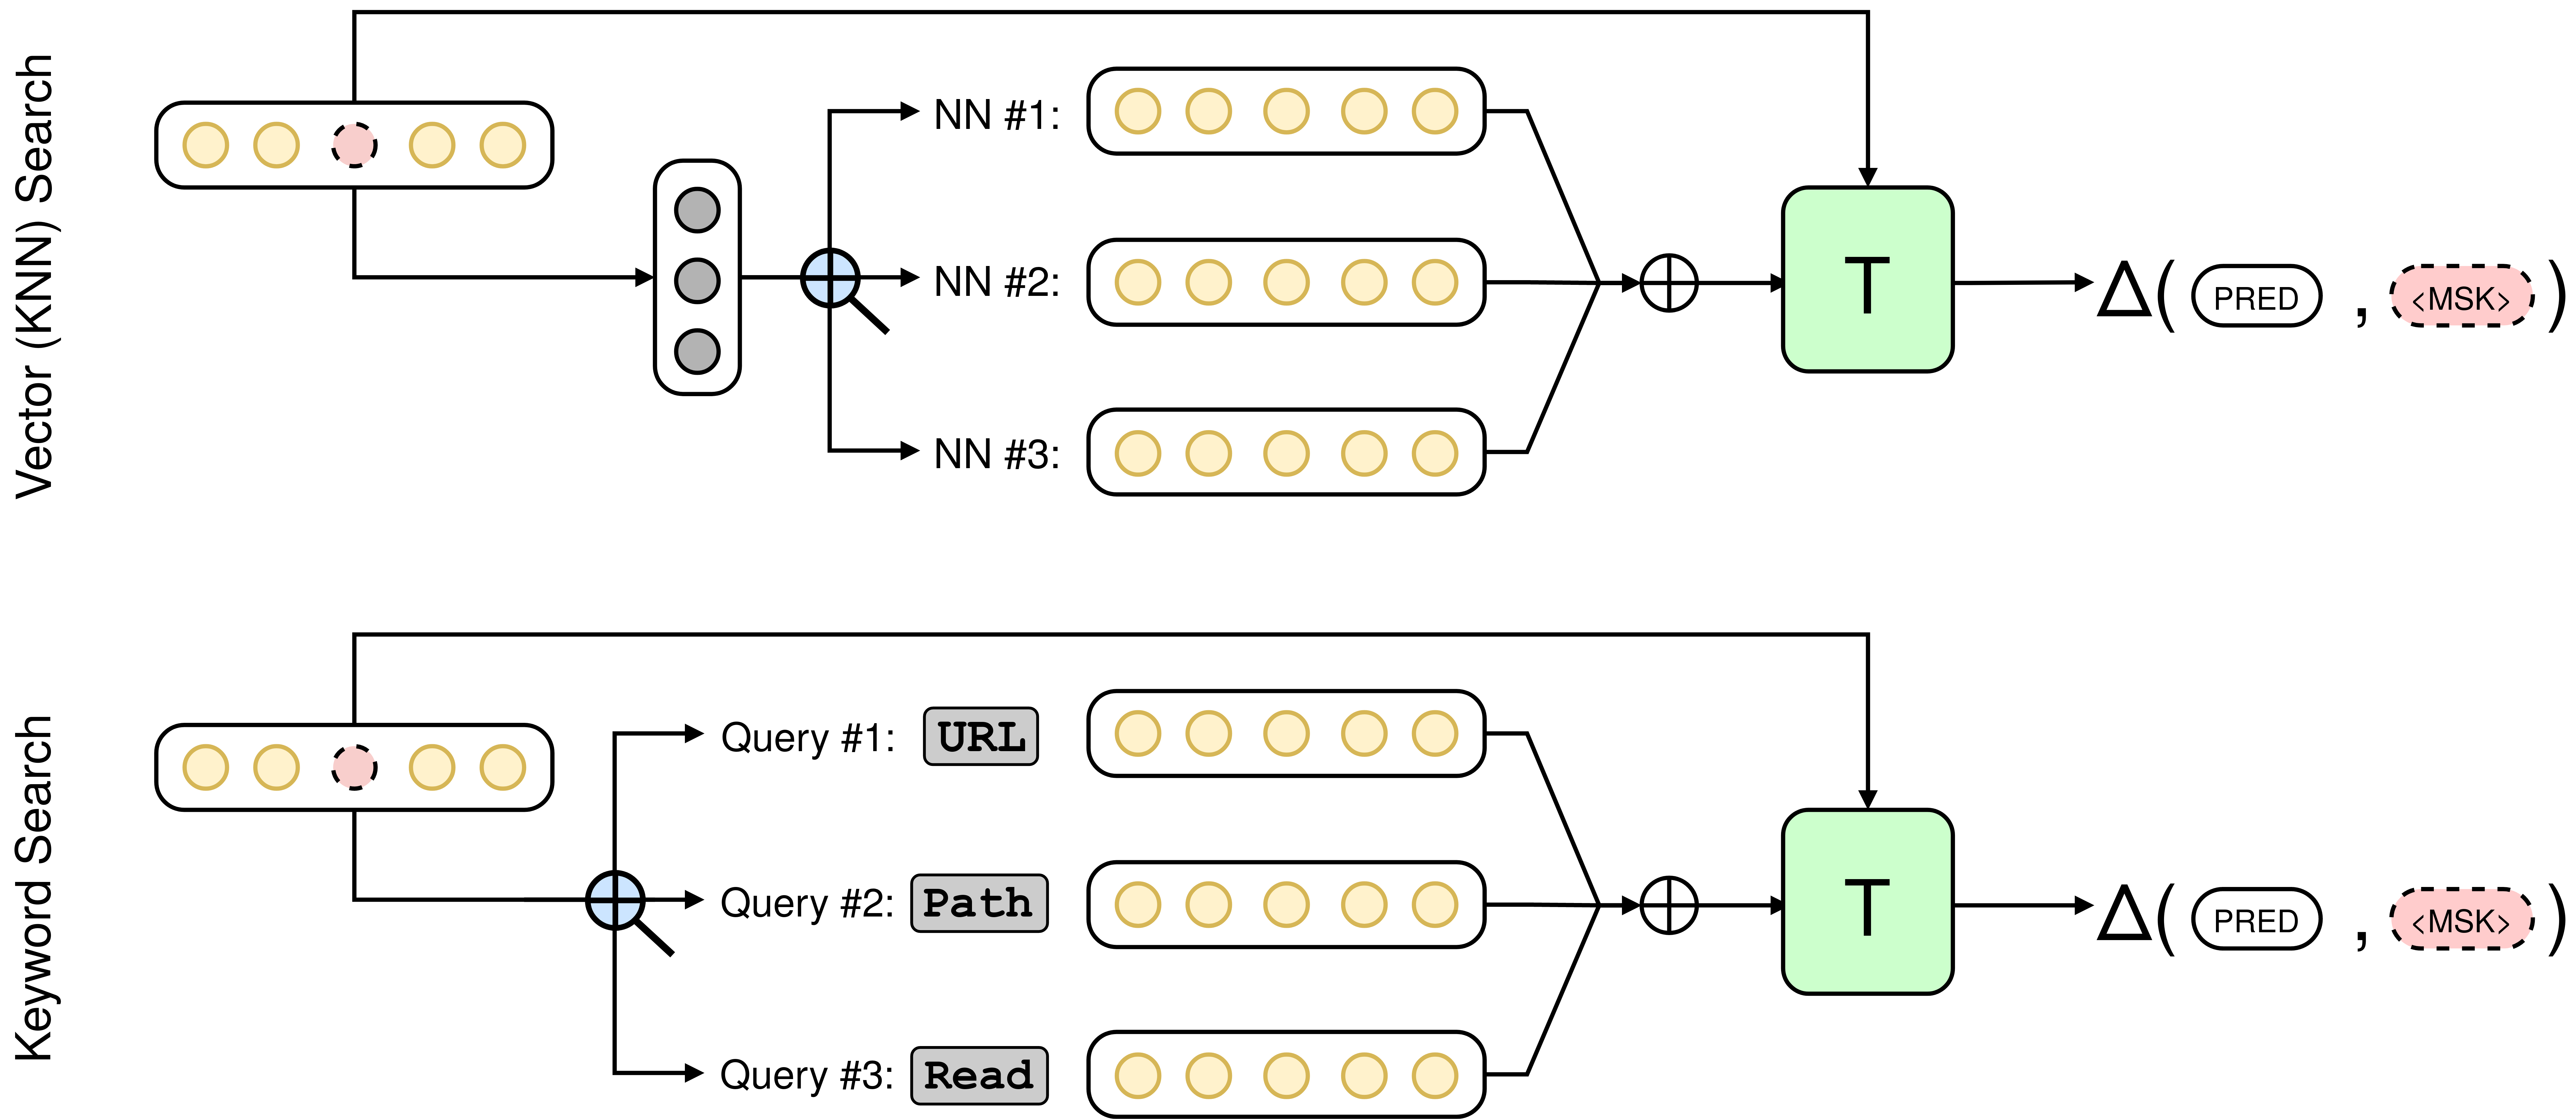
\includegraphics[width=0.4\textwidth]{figs/knn_vs_vec}
    \caption{In the vector search procedure, we compute an embedding for the masked source context, then retrieve the k-nearest sequence embeddings in our database. In the keyword search, we compute an n-hot vector to select the keywords, and retrieve the nearest matching sequences in our index. In both cases, we embed the results, feed them into a transformer, compute a loss between the predicted output and the masked token, and backpropagate.}
    \label{fig:pipeline}
  \end{figure}

  Once the beam search procedure is complete, we have a graph representing the neighborhood of the nearest neighboring code fragments in the parent project. This forms a so-called \textit{virtual knowledge graph}, with nodes decorated by the CodeBERT sequence embeddings and edges decorated with the direction vector between documents. We then run $p$ rounds of message passing to obtain graph embedding or \textit{neighborhood summary vector} (Fig.~\ref{fig:architecture}).

% We initialize the policy network using a pretrained language model. Starting at the site of the prediction task and conditioning on its local context, the policy network draws K queries from its latent state, which are fed into the index to produce a set of matching locations. The model scores and selectively expands a subset of those locations, and the process is repeated using finite-horizon MCTS or similar beam search procedure to retrieve a set of contextually relevant locations within the parent project.
%
%The rollout traces form a graph of related locations inside each project and their corresponding context embeddings, which together form the GNN node features. Once the rollout ends, we run message passing on the resulting GNN for a fixed numbers of steps and decode the graph embedding to obtain a task prediction. The decoder, GNN parameters, and policy network are all trained end-to-end on the downstream task, e.g. code completion, defect detection or correction. After convergence, we compare the results across horizon size and analyze the queries and filetypes which are selected.

  \pagebreak
  \section{Experiments}\label{sec:experiments}

  In this work, we attempt to understand the relationship between entities in a software project. Our research seeks to answer the following questions:

  \begin{enumerate}
    \item Which contexts in a software project share mutual information?
    \item To what degree can we claim the model has learned to:\begin{enumerate}
                                                                 \item Locate contextually relevant artifacts within a software project?
%   \item Comprehend the semantic content of the artifacts traversed?
%   \item Apply the knowledge gathered to perform the assigned task?
    \end{enumerate}
  \end{enumerate}

  {
    \renewcommand{\arraystretch}{1.5}
    \begin{table}[H]
      \small
      \begin{tabular}{l|ccc}
        Model & IRA & QDL & P/R \\
        \hline
        \href{https://huggingface.co/microsoft/CodeGPT-small-java}{\textsc{CodeGPT}}~\citep{lu2021codexglue} & X & X & X \\
        \href{https://huggingface.co/microsoft/graphcodebert-base}{\textsc{GraphCodeBERT}}~\citep{guo2021graphcodebert} & X & X & X \\
        \href{https://huggingface.co/huggingface/CodeBERTa-small-v1a}{\textsc{CodeBERT-small}}~\citep{feng2020codebert} & X & X & X \\
        \href{https://huggingface.co/dbernsohn/roberta-java}{\textsc{RoBERTa-Java}}~\citep{liu2019roberta} & X & X & X \\
        \href{https://copilot.github.com/}{\textsc{Copilot}}\citep{chen2021evaluating} & X & X & X \\

      \end{tabular}
      \caption{\label{tab:ad_comparison} Experiments table for comparing pretrained LM embeddings on source code snippets. IRA: Iterrater agreement. QDL: query description length, P/R: Precision/recall}
    \end{table}
  }


  For each of these models (available on HuggingFace), we sample a set of code snippets from our synthetic dataset, and compare how well they agree on each task.


  In contrast with classical code completion models which only require a file-local context, our method is designed to navigate an entire project. In the following experiments, we compare completion accuracy with a vanilla sequence prediction model, as well as an AST-structured sequence prediction model trained from a corpus of Java projects on the same task.

  We hypothesize that by jointly learning to choose locations in a project over which to attend while solving a downstream task, such as masked sequence completion, our model will produce a feature representation capable of locating and extracting information from semantically relevant contexts. We evaluate our hypothesis both qualitatively and quantitatively.

  In our first set of experiments, we try to understand what is shared between sequences mapped to similar latent vectors. Do similar sequences share salient keywords? Are those keywords relevant to the task?

  In our second experiment, we try to measure the information gain from including and excluding various filetypes through ablation. For graphs containing filetypes which include Markdown or Java, what kinds of information do these resources provide and which categories are most salient?

%In our third experiment, we compare prediction accuracy across architectures and datasets. Can we constrain the action space (e.g. only querying tokens from the surrounding context) for more efficient trajectory sampling, or allow arbitrary queries? How well does the model architecture transfer to new repositories, within and across programming languages?

  In our third and final set of experiments, we compare performance across hyperparameters. Does contextual expansion lead to better task performence for a given sequence prediction task? By relaxing edge-construction criteria and increasing hyperparamers such as beam search budget, we would expect corresponding task performance to increase.

  If our hypothesis is correct, the virtual knowledge graph will span both natural language and source code artifacts. If so, this would provide evidence to support the broader hypothesis~\citep{guo2017semantically} that documentation is a useful source of information. In addition to being useful for the prediction task itself, we anticipate our model could also be used for knowledge graph extraction and suggest semantically relevant code snippets to developers.



  \pagebreak
  \section{Evaluation}\label{sec:evaluation}

  We evaluate on the following loss function, adapted from~\citep{husain2019codesearchnet}. Given a set of code and context pairs, $\mathbf{F} = (\mathbf{c}_i, \mathbf{d}_i)_{i = 1}^N$, where $\mathbf S \sim_{i.i.d.} \mathbf R_{d}$:

  \begin{align}
    \mathcal{L} = \frac{1}{N}\sum_i^N \log\left(\frac{\left<\varphi(\mathbf{c}_i), \varphi(\mathbf{d}_i)\right>}{\sum_{j \neq i}^N \left<\varphi(\mathbf{c}_j), \varphi(\mathbf{d}_i)\right>}\right)
  \end{align}

  In other words, we minimize the distance between true code and context pairs, while maximizing the distance between distractors $(\mathbf c_j, \mathbf d_i)_{i \neq j}$.

%\section{Next steps}
%
%Our next steps are to build a simple environment which allows an agent to interact with a software repository and construct a graph. We will use an in-memory filesystem to store and load project artifacts. The policy network will need to be pretrained on a corpus of projects in the same language. To model the action space, we will use the radix tree of the parent project, with transition probabilities conditioned on the local context.
%
%For further details and to get started, please visit our GitHub page: \url{https://github.com/breandan/gym-fs}.

  \pagebreak
  \section{Results}\label{sec:results}

  Our preliminary results compare distance metrics (Fig.~\ref{fig:lev_vs_euclid}), explore embedding quality (Fig.~\ref{fig:embedding}) and visualize the synthetic knowledge graphs (Fig.~\ref{fig:graphs}).

  \begin{figure}[H]
    \centering
    \begin{tikzpicture}
      \begin{axis}[width=0.29\textwidth, height=0.3\textwidth, xlabel=Levenshtein, ylabel=Euclidean]
        \addplot table [mark=none,x=strdist, y=embdist, variable=var, col sep=comma] {data/levenshtein.csv};

        \addplot [smooth, name path=upper,draw=none] table[x=strdist, y=embdist,variable=var, y expr=\thisrow{embdist}+\thisrow{var}, col sep=comma] {data/levenshtein.csv};
        \addplot [smooth, name path=lower,draw=none] table[x=strdist, y=embdist,variable=var, y expr=\thisrow{embdist}-\thisrow{var}, col sep=comma] {data/levenshtein.csv};
        \addplot [fill=red!10] fill between[of=upper and lower];
      \end{axis}
    \end{tikzpicture}
    \begin{tikzpicture}
      \begin{axis}[width=0.29\textwidth, height=0.3\textwidth, xlabel=Damerau]
        \addplot table [mark=none,x=strdist, y=embdist, variable=var, col sep=comma] {data/damerau.csv};

        \addplot [smooth, name path=upper,draw=none] table[x=strdist, y=embdist,variable=var, y expr=\thisrow{embdist}+\thisrow{var}, col sep=comma] {data/damerau.csv};
        \addplot [smooth, name path=lower,draw=none] table[x=strdist, y=embdist,variable=var, y expr=\thisrow{embdist}-\thisrow{var}, col sep=comma] {data/damerau.csv};
        \addplot [fill=red!10] fill between[of=upper and lower];
      \end{axis}
    \end{tikzpicture}
    \begin{tikzpicture}
      \begin{axis}[width=0.29\textwidth, height=0.3\textwidth, xlabel=MetricLCS]
        \addplot table [mark=none,x=strdist, y=embdist, variable=var, col sep=comma] {data/metriclcs.csv};

        \addplot [smooth, name path=upper,draw=none] table[x=strdist, y=embdist,variable=var, y expr=\thisrow{embdist}+\thisrow{var}, col sep=comma] {data/metriclcs.csv};
        \addplot [smooth, name path=lower,draw=none] table[x=strdist, y=embdist,variable=var, y expr=\thisrow{embdist}-\thisrow{var}, col sep=comma] {data/metriclcs.csv};
        \addplot [fill=red!10] fill between[of=upper and lower];
      \end{axis}
    \end{tikzpicture}
    \begin{tikzpicture}
      \begin{axis}[width=0.29\textwidth, height=0.3\textwidth, xlabel=Jaccard]
        \addplot table [mark=none,x=strdist, y=embdist, variable=var, col sep=comma] {data/jaccard.csv};

        \addplot [smooth, name path=upper,draw=none] table[x=strdist, y=embdist,variable=var, y expr=\thisrow{embdist}+\thisrow{var}, col sep=comma] {data/jaccard.csv};
        \addplot [smooth, name path=lower,draw=none] table[x=strdist, y=embdist,variable=var, y expr=\thisrow{embdist}-\thisrow{var}, col sep=comma] {data/jaccard.csv};
        \addplot [fill=red!10] fill between[of=upper and lower];
      \end{axis}
    \end{tikzpicture}  \caption{CodeBERT latent space distance correlates with string edit distance.}
    \label{fig:lev_vs_euclid}
  \end{figure}

  \begin{figure}[H]
    \centering
    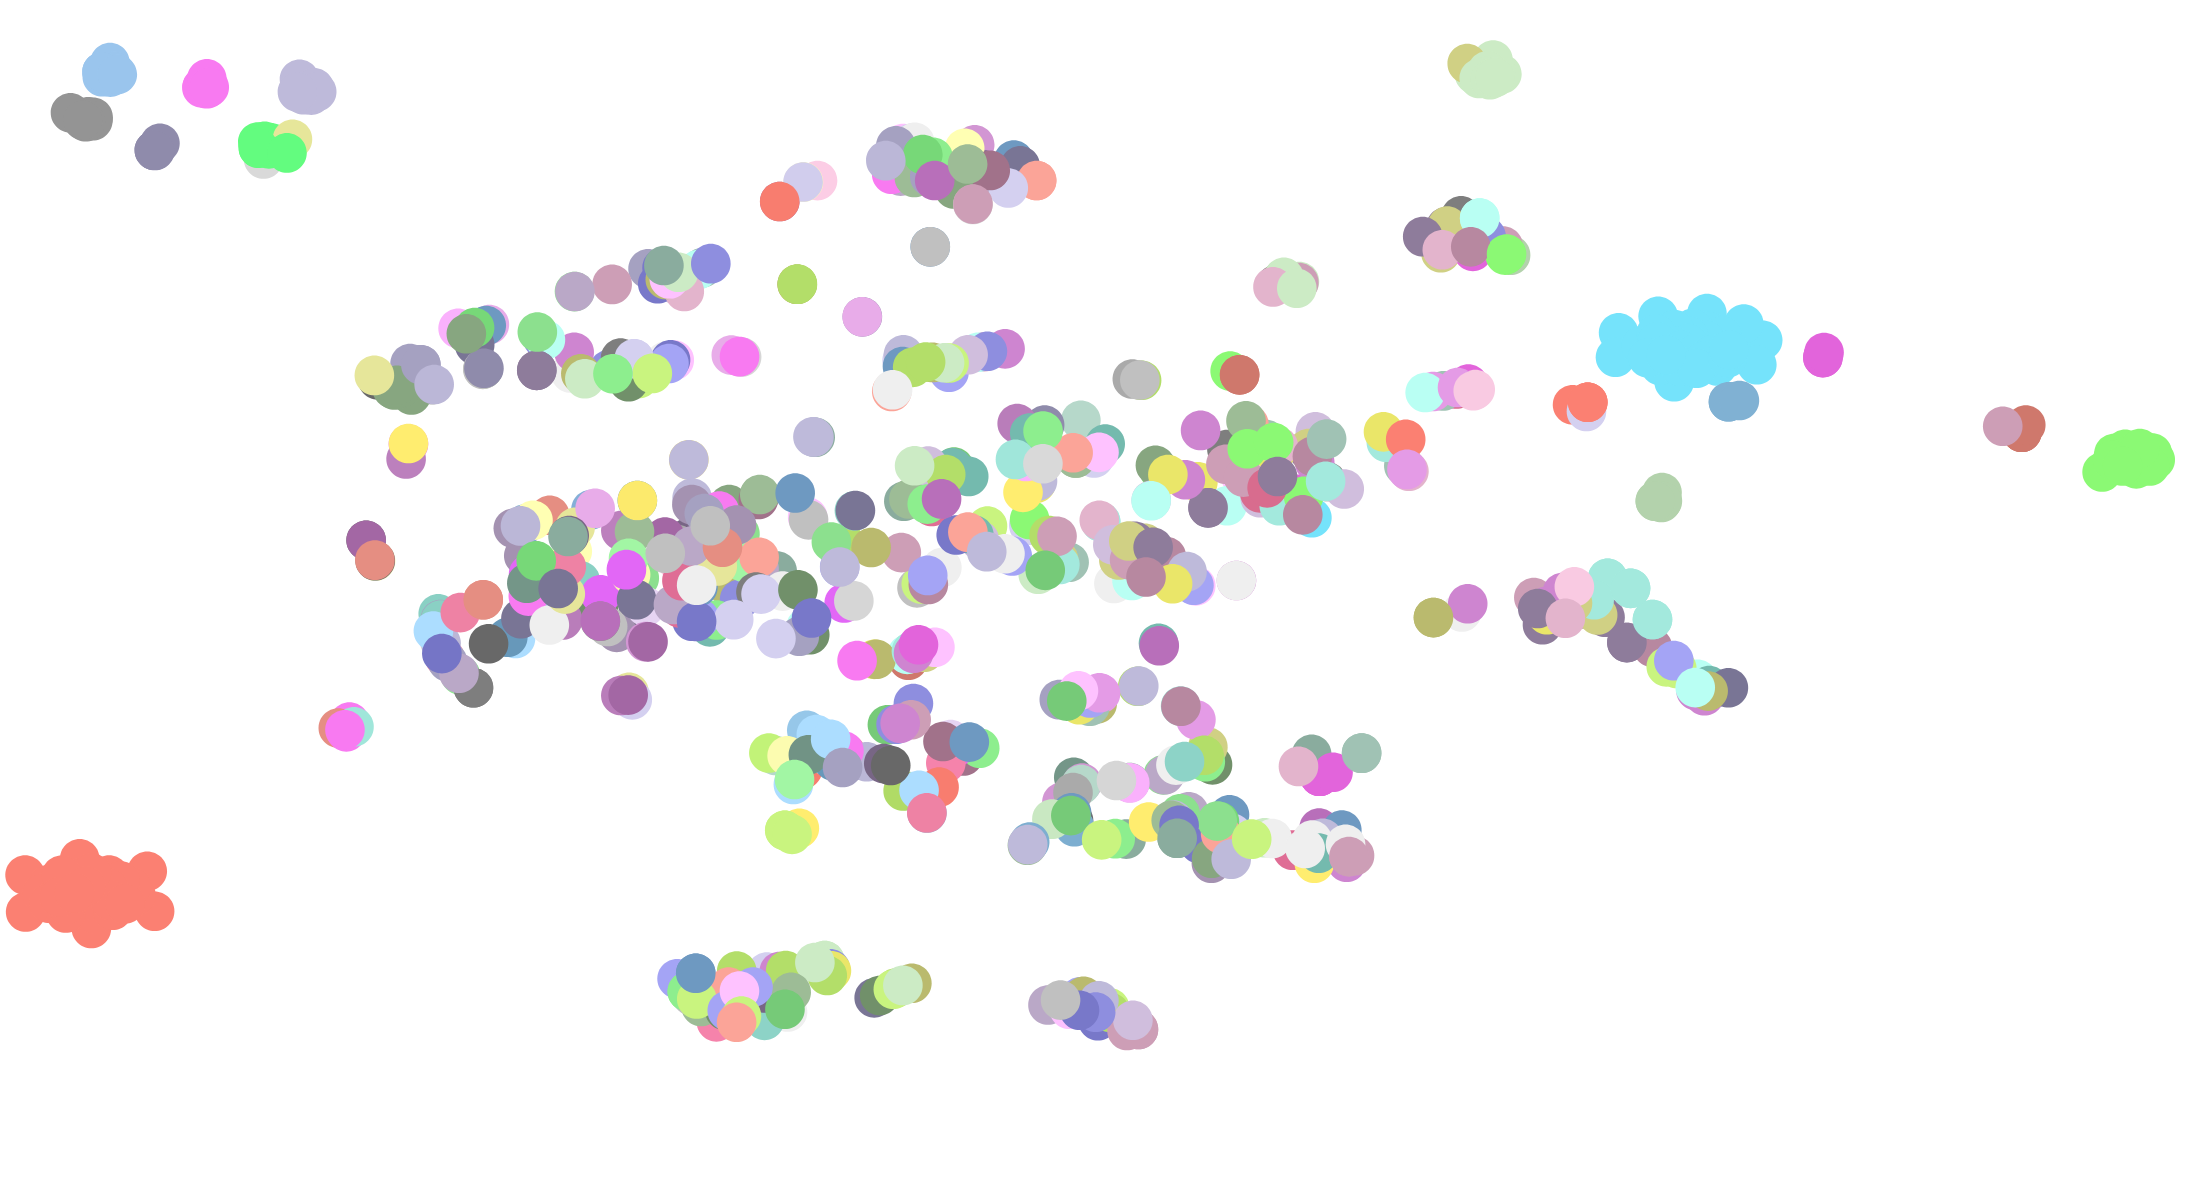
\includegraphics[width=0.4\textwidth]{figs/embeddings}
    \caption{Reduced dimensionality TNSE embeddings colored by line length.}
    \label{fig:embedding}
  \end{figure}

  \begin{figure}[H]
    \centering
    \resizebox{.2\textwidth}{!}{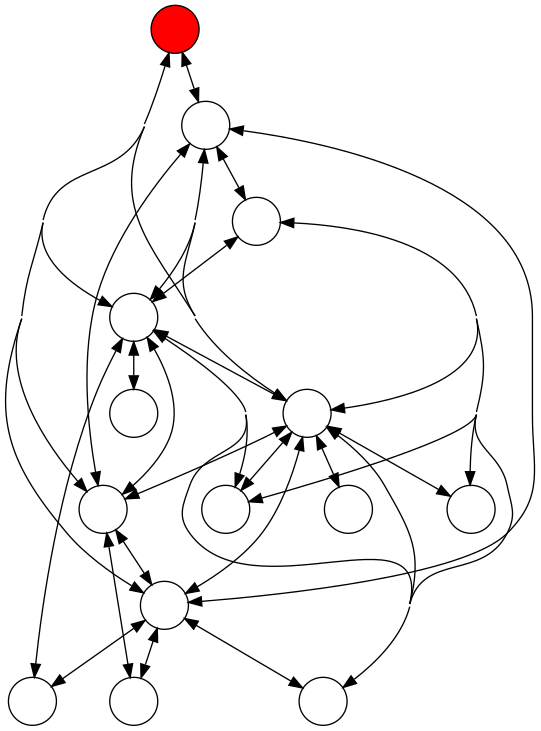
\includegraphics{data/query4}}
    \resizebox{.2\textwidth}{!}{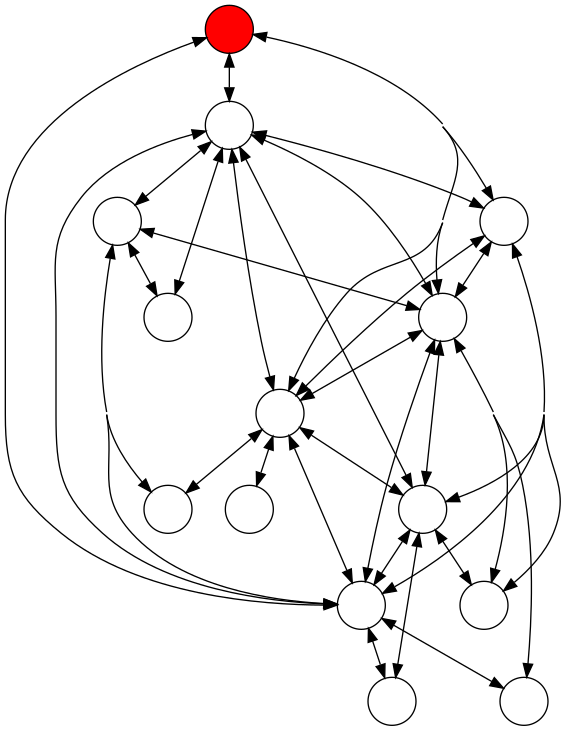
\includegraphics{data/query5}}
    \resizebox{.2\textwidth}{!}{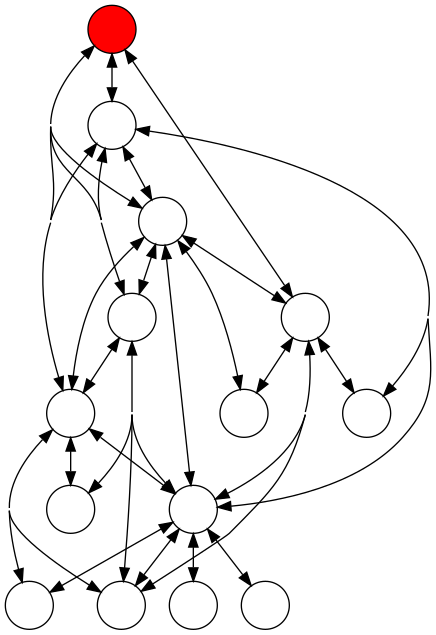
\includegraphics{data/query6}}
    \resizebox{.2\textwidth}{!}{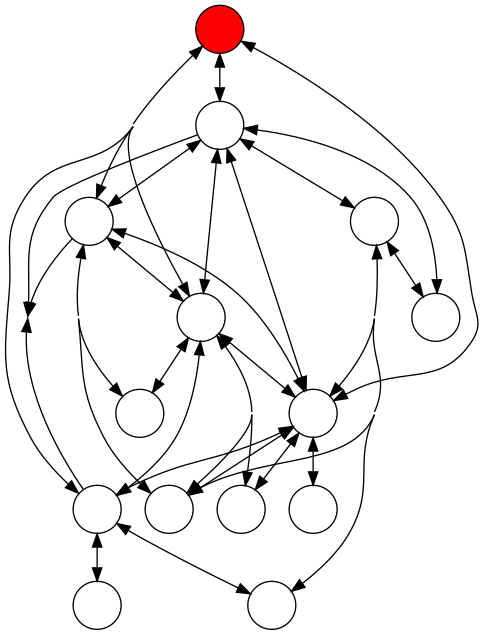
\includegraphics{data/query7}}
    \resizebox{.2\textwidth}{!}{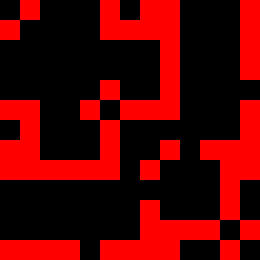
\includegraphics{data/context4}}
    \resizebox{.2\textwidth}{!}{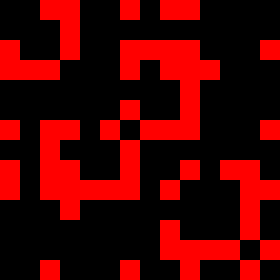
\includegraphics{data/context5}}
    \resizebox{.2\textwidth}{!}{
\includegraphics{data/context6}}
    \resizebox{.2\textwidth}{!}{
\includegraphics{data/context7}}
    \caption{Example graphs sampled by beam search with $d=10, w=5$.}
    \label{fig:graphs}
  \end{figure}
  \bibliography{main}
  \bibliographystyle{plain}

\end{document}
\endinput
%%
%% End of file `sample-sigconf.tex'.